%
% File acl2010.tex
%
% Contact  jshin@csie.ncnu.edu.tw or pkoehn@inf.ed.ac.uk
%%
%% Based on the style files for ACL-IJCNLP-2009, which were, in turn,
%% based on the style files for EACL-2009 and IJCNLP-2008...

%% Based on the style files for EACL 2006 by 
%%e.agirre@ehu.es or Sergi.Balari@uab.es
%% and that of ACL 08 by Joakim Nivre and Noah Smith

\documentclass[11pt]{article}
\usepackage{polyglossia}
\setmainlanguage{english}
\setmainfont[Mapping=tex-text]{Times New Roman}
\usepackage{acl2010}
%\setmainfont{TeX Gyre Termes}
%\usepackage{times}
\usepackage{url}
\usepackage{latexsym}
\usepackage{graphicx}
\usepackage{enumitem}
\usepackage[hidelinks]{hyperref}
\usepackage{omwmacros}
%\setlength\titlebox{6.5cm}    % You can expand the title box if you
% really have to
\usepackage[round]{natbib}
\newcommand{\lex}[1]{\textbf{\textit{#1}}}
\title{Linking the TUFS Basic Vocabulary \\ to the Open Multilingual Wordnet}

\author{
	Francis Bond,$^\spadesuit$ 
	Hiroki Nomoto ,$^\diamondsuit$
	Luis Morgado da Costa$^\spadesuit$\\
  $^\spadesuit$ Nanyang Technological University (NTU),  Singapore\\
  $^\diamondsuit$
  Tokyo University of Foreign Studies (TUFS), Japan \\
  \url{bond@ieee.org, nomoto@tufs.ac.jp} }

\date{}

\begin{document}
\maketitle
\begin{abstract}
We describe preliminary work in the creation of the first specialized vocabulary to be integrated into the Open Multilingual Wordnet (OMW). The NCIt Derived WordNet (ncitWN) is based on the National Cancer Institute Thesaurus (NCIt), a controlled biomedical terminology that includes formal %description logic 
class restrictions and English definitions  developed by groups of clinicians and terminologists. The ncitWN is created by converting the NCIt to the WordNet Lexical Markup Framework and adding semantic types. We report the development of a prototype ncitWN and first steps towards integrating it into the OMW.
\end{abstract}
\section{Introduction}
%TODO - FB, Can you decide where to use GWG and OMW? 
The Global Wordnet Grid (GWG) is a platform created to join together wordnets by linking them to a central registry of concepts, using the Collaborative Interlingual Index (CILI) as a pivot.  Data in the GWG is linked following an `onion model', with `a core of concepts shared by many wordnets', validated by the community, and axiomatized through ontologies. The core extends to a middle layer with fewer shared wordnets and out to a layer of concepts mapped to only a single wordnet. An external layer contains synsets defined in project wordnets that do not fulfill the CILI inclusion criteria. One of the advantages of the GWG is that the resource is no longer limited to networks of single-word units, but is now open to phrasenets (frequent adjective-noun, noun-prep-noun, and verb-object combinations, as well as proverbs, idioms, and compounds). This feature creates the possibility to link wordnets to domain-specific terminologies, which often include multi-word expressions.  The Open Multilingual Wordnet (OMW) is the reference instantiation of the GWG \citep{Bond:2016a} adding the constraint that all member wordnets must be open according to the open definition.\footnote{The Open Definition, \url{http://opendefinition.org} (October~28, 2017).}

To date no specialized terminologies have been included in the OMW. Consequently, there is no established procedure for mapping technical concepts to the CILI nor for determining whether a technical concept ought to be indexed in the CILI. We report a preliminary biomedical wordnet based on the National Cancer Institute Thesaurus (NCIt) called the NCIt Derived Wordnet (ncitWN) and preliminary mappings to the CILI. By mapping the NCIt to the CILI and thereby integrating it into the OMW, we are developing the first specialized vocabulary mapped to the CILI. The two outcomes will be: (i) the NCIt mapped to the CILI and integrated into OMW, but just as significantly (ii) groundwork for a method to reliably integrate open and freely available specialized terminologies with these lexical resources. This work is a first step toward realizing the goals outlined in \citet{smith2004medical}.

\section{Resources}

\subsection{The Collaborative Interlingual Index}
The CILI is implemented as a collaborative open-source software based on the best-practices of the Semantic Web -- persistent IDs, Creative Commons Attribution 4.0 (CC BY) license allowing redistribution, and versioning \citep{Bond:2016a}. It integrates and extends the list of concepts in the OMW, including all concepts in Princeton WordNet of English (PWN) \citep{Fellbaum:1998a}. Each concept in the CILI is described with a unique definition in English. Currently, most of these definitions are derived from PWN~3.0. The CILI is compatible with the two schemas (Wordnet-LMF/lemon) \citep{vossen2016toward,mccrae2014publishing}
used for encoding individual wordnets. The Semantic Web identifiers conform to the standards being adopted for encoding and integrating biomedical terminologies and ontologies \citep{ruttenberg2007advancing,schuurman2008ontologies} and allow the CILI to be linked to ontologies and domain-specific terminologies.  The CILI's open collaborative framework includes rules, tools, and safeguards to support high quality, agreed-upon mappings of wordnets to the CILI \citep{Bond:2016a}.

\subsection{Princeton Wordnet}

In order to get lemmas and domain information for English, we use the Princeton WordNet of English 3.0 \citep{Fellbaum:1998a}. Synsets are grouped into 45 \textbf{lexicographer files} which we use as coarse domains (for example, \texttt{noun.artifact} contains   nouns denoting man-made objects).  PWN also has explicit domains linked by the \texttt{domain-category} relation, which we intend to use in future work.

\subsection{The National Cancer Institute Thesaurus and the UMLS Metathesaurus}
The NCIt is a reference terminology developed by the National Cancer Institute that covers over 118,000 concepts and is available in the Web Ontology Language (OWL)~\citep{sioutos2007nci}. Although initially developed to support research and data management in the domain of cancer, it also includes concepts of general biomedical interest that are not specific to cancer, such as a robust typology of diseases, procedures, and adverse events. Each concept in the NCIt is associated with a unique identifier, a preferred term, and synonyms. Many terms also include an English definition, a description logic definition, and cross-references to other terminologies. The English definitions are developed by groups of clinicians and terminologists. The clinicians are often from the international English speaking community (USA, UK, Australia). The NCIt is released under a special license. We communicated with the creators and maintainers and have ensured that the ncitWN and its inclusion in the GWG is in compliance with their license.\footnote{NCI THESAURUS Terms of Use, \url{https://evs.nci.nih.gov/ftp1/NCI_Thesaurus/NCI_THESAURUS_license.txt} (October 28, 2017).} Terms are also classified using the  Unified Medical Language System (UMLS) Semantic Types: there are 127 semantic types linked in an is-a hierarchy. 

The NCIt is included in the Unified Medical Language System Metathesaurus, a biomedical thesaurus that links approximately 200 biomedical terminologies to an index of concepts \citep{schuyler1993umls}. In this respect, the UMLS Metathesaurus can be viewed as a domain specific analogue of the Open Multilingual Wordnet (OMW). The UMLS Metathesaurus also includes translations of some of its source vocabularies into languages other than English. It is available in two data formats, the Rich Release Format and the Original Release Format. Semantic types such as ``Drug'' have been added to the UMLS Metathesaurus to impose more structure and to organize concepts \citep{NLM:2009}.

\subsection{Wordnet-Lexical Markup Framework}
Wordnet-Lexical Markup Framework is a wordnet-implementation of the Lexical Markup Framework \citep{francopoulo2006lexical} (LMF), an ISO standard for NLP lexicons and Machine Readable Dictionaries based on the eXtensible Markup Language (XML) format. It encodes linguistic knowledge of the lexicalized concepts represented in the wordnets and supports integration of wordnets with OMW \citep{da2015omwedit,Vossen:2013b,Bond:Foster:2013}. Although no domain specific resources have been integrated into the CILI to date, this schema is well suited for the integration of an external resource such as the NCIt. 
Wordnet-LMF allows for a greater inventory of semantic relations than the NCIt currently contains, including entailment, part-whole relations, and derivations.

\section{Methods}

\subsection{Convert NCIt to Wordnet-LMF} 

We have written a simple program (in Python~3) to reformat the NCIt as a wordnet (ncitWN).  It filters out obsolete and retired concepts, creates the necessary metadata, and builds a wordnet.  The conversion process is based on a few assumptions, to be tested further: (1) all concepts are lexicalized as nouns, and (2) the child-parent relationship in the thesaurus can be modeled as simple hypernymy.

The UMLS Semantic Types could be modeled as external links or as links within the wordnet (as PWN does).  Currently we add them as metadata on each synset (using \texttt{dc:type}).

We  validate the ncitWN data format with (1) the LMF Document Type Definition, which validates the XML representation of the Wordnet-LMF documents \citep{vossen2016toward} and (2) the OMW’s online tool \citep{da2015omwedit,tan2011building} that detects content violations such as duplicate or missing definitions.

\subsection{Map ncitWN to the CILI} % - AH and SS
We have tested the feasibility of mapping the ncitWN to the CILI using two approaches. 

The first, automatic, approach uses the prototype Wordnet-LMF formatted version of NCIt to automatically generate candidate mappings to the CILI using lemma overlap and compatibility of UMLS Semantic Types with WordNet coarse domains.  The score is the sum of the Jaccard similarity calculated over lemma overlap with a boost of 0.1 each time there is a match between the wordnet coarse domains and the UMLS Semantic Type, based on a simple table of equivalences.

For example consider the following match:
\begin{itemize}
\item \lex{mask} (NCIt) ``A protective covering worn over the face, or an apparatus for administering anesthesia or oxygen through the nose or mouth'' «Manufactured Object» (C86570)
\item \lex{mask}$_{n:4}$ (PWN) ``a protective covering worn over the face'' «noun.artifact» (\ili{i56041})
\end{itemize}
Here the overlap in lemmas is 100\% (\{\lex{mask}\} vs. \{\lex{mask}\}) and «Manufactured Object» matches «noun.artifact» so the score is 1.1.  The equivalence table was made by first matching %using 
only lemmas and, assuming that all 100\% matches were good, linking the UMLS Semantic Type and PWN coarse domain. All matches of semantic types with more than 500 examples were taken to be good.   An inspection of the less frequent matches showed many to be good, this mapping should be revised in subsequent work.

We manually evaluated a sample of the automatically produced matches with a match score $>$~.75. The annotation scheme is summarized in Table~\ref{tab:annotation}.
`0' is not used for mapping, but was nevertheless used to annotate candidate matches. These annotations will be used to generate heuristics for refining match scores, thereby expediting the mapping process.

\begin{table}[h]
\begin{center}
\begin{tabular}{|l|l|}
\hline \bf Annotation & \bf Meaning \\
\hline eq &  equivalence \\
spec &  hyponym of  \\
gen &    hypernym of\\
0 & no hierarchy relation \\
\hline
\end{tabular}
\caption{Annotations for candidate matches from ncitWN synset to PWN synset}\label{tab:annotation}
\end{center}
\end{table}

Note that an annotation of `0' does not indicate that there is no relation between the NCIt and PWN term, but only that there is no hierarchical relation. There might be non-hierarchal relations, e.g., linguistically derived from, that may be incorporated in future work.

The second approach was a manual analysis of PWN~3.0's coverage of the NCIt. We randomly selected 94 concepts from the NCIt, stratified according to whether the concept was a root, middle, or leaf node (respectively, 19, 37, and 38 concepts). We then searched for candidate mappings through lemmas in PWN and evaluated the match based on the corresponding definitions in the CILI. The manual coverage analysis was based on NCIt preferred terms and excludes synonyms. Preferred terms that take the form of boolean expressions such as `Diagnostic or Prognostic Factor' were decomposed into their component expressions, which were used for searching candidate mappings. Thus, for `Diagnostic or Prognostic Factor', we restored the elliptical noun and obtained two multiword expressions (MWEs) for which we searched candidate mappings, i.e., `Diagnostic Factor' and `Prognostic Factor'. 

We distinguish six matching scenarios summarized in Table~\ref{Manual_annotations} and illustrate them with examples below.
\begin{table}[h]
\begin{center}
\begin{tabular}{|l|l|}
\hline \bf Annotation & \bf Meaning \\
\hline 
0 & no match%: neither the full NCIt lemma nor any part of it matches a PWN lemma and/or the definitions don't match 
\\
1 & exact match%: the NCIt and PWN lemmas and the corresponding NCIt and ILI definitions match
\\
2 & full match%: each word of an NCIt MWE has a compositionally matching PWN lemma and ILI definition
\\
3 & partial match of MWE%: at least one word of an NCIt MWE has a compositionally matching PWN lemma and ILI definition 
\\
4 & preferred term with partial match%: the definition of the NCIt preferred term has a partially matching ILI definition %, i.e., the NCIt definition is more specific or broader than the ILI definition. Does not apply to elements of boolean terms or of MWEs. 
\\
5 & not suitable to map to CILI
\\
\hline
\end{tabular}
\caption{\label{Manual_annotations}Annotation scheme for candidate matches from NCIt terms to PWN synsets}
\end{center}
\end{table}

The coverage analysis was carried out in several steps (see Figure~\ref{steps}). 
In step~1, we determined whether the NCIt preferred term had a match in the PWN lemmas. If it did not, we annotated it with `0'. %For example, `Archaea' (C61092) was not found in PWN and was thus assigned the label `0'.
If there was a match, in step~2, we compared the NCIt and CILI definitions. If both the lemmas and the definitions matched, we considered them an exact match (`1'); if the lemmas matched but the NCIt definition was either more specific or broader than the CILI definition, the NCIt preferred term has a partial map (`4'); if the NCIt term and definition were NCI-specific, the concept was not suitable to be mapped to the CILI (`5'). If none of these options applied and the NCIt term was an MWE, in step 4, we decomposed the MWE into its parts and searched each word individually. In case of a match, we determined whether the CILI definition for the matched PWN lemma corresponds to the compositional meaning of the word in the NCIt MWE. If the meaning and the definition matched, we assigned `1',  otherwise `0'. In step~5, we assigned an annotation to the NCIt preferred MWE by considering all the individual annotations assigned to each word composing the MWE.

\begin{figure*}[h]
\centering
 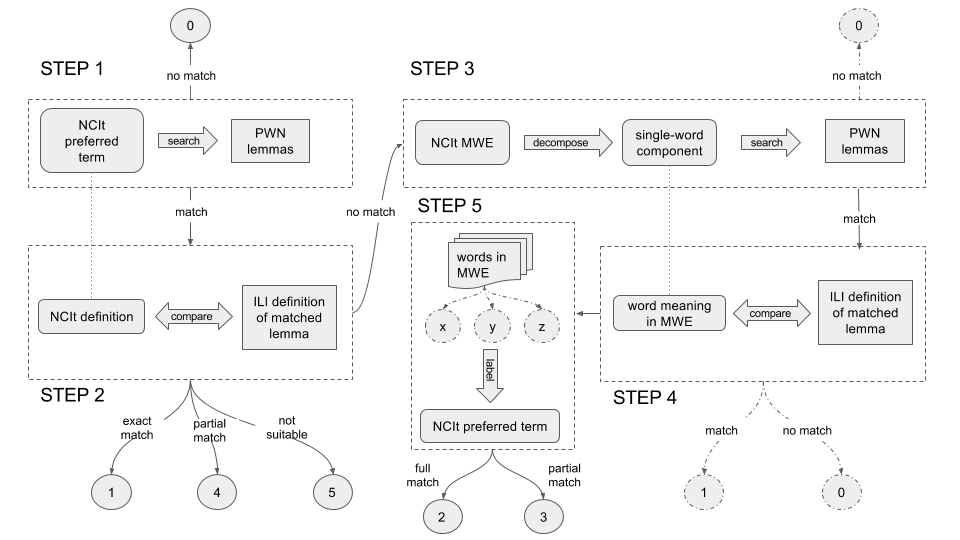
\includegraphics[scale=.4]{NCIt-ILI_manual_mapping} % width=\textwidth
 \caption{Steps of the manual coverage analysis}
\label{steps}
\end{figure*}

Examples of matching and non-matching cases:
\begin{enumerate}[start=0]
\item NCIt \lex{Archaea} (C61092) is not in PWN.
\item NCIt \lex{Area} (C25244) and PWN \lex{area}$_{n:6}$ (\ili{i63937}) have identical definitions.
\item NCIt \lex{Breast Cancer Prognostic Factor} (C19601) has no exact match in PWN but its parts do. The individual annotations assigned to each matched part of the MWE (`breast cancer': 1; `prognostic': 1; `factor':~1) allow us to assign the global annotation `2' to the preferred term.
\item NCIt \lex{Ito Cell Tumor} (C80350) has no exact match in PWN and only two out of the three words composing the MWE are in PWN with the same meaning (`cell': 1; `tumor': 1; `ito': 0). These individual annotations allow us to assign the annotation `3' to the preferred term.
\item NCIt \lex{Acclimatization} (C68767), defined as ``The physiological process through which an organism grows accustomed to a new environment'', has a narrower definition than the CILI definition corresponding to PWN \lex{acclimatization}$_{n:1}$,``adaptation to a new climate (a new temperature or altitude or environment)'' (\ili{i107289}).
\item NCIt \lex{NCI Administrative Concept} (C28389) and its definition %(``An entity which is used by NCI for administrative, financial or organizational purposes'' 
are specific to the NCI, therefore not suitable for mapping to the CILI.
\end{enumerate}
% [EXAMPLES]
% 1: `Area' (C25244) The extent of a 2-dimensional surface enclosed within a boundary. - `area' (i63937) the extent of a 2-dimensional surface enclosed within a boundary
% 2: `Breast Cancer Prognostic Factor' (C19601): A situation, condition, or a characteristic of a patient that can be used to estimate the chance of recovery from breast cancer or the chance of recurrence of breast cancer. -> breast cancer=1, prognostic=1, factor=1, global=2
% 3: `Ito Cell Tumor' (C80350) A benign or malignant tumor of the liver composed of hepatic stellate cells. -> cell=1, tumor=1, ito=0, global=3
% 4: `Acclimatization' (C68767) The physiological process through which an organism grows accustomed to a new environment. - `acclimatization' (i107289) adaptation to a new climate (a new temperature or altitude or environment) -> ILI definition is broader 
% !!! 4: The following are labeled 4 and are contrary to the specifications for 4: `body substance' in `Body Fluid or Substance'; `abnormality' in `Protein Splicing Abnormality'.
% 5:`NCI Administrative Concept' (C28389) -> a concept specific to the NCIt, therefore not suitable for mapping to ILI.



%TODO: As part of the UMLS, NCIt is mapped to UMLS Semantic Types,72 which have been added to the UMLS to help disambiguate and cluster senses. Similarly, PWN contains domain-category links such as <tobacco is in the domain of pharmacy>. Dr. Amanda Hicks (PI) will manually map the UMLS Semantic Types and WordNet domain-category types and add WordNet domain-category types to the ncitWN where there is no existing type corresponding UMLS Semantic Type. This will enrich the overall graph in ncitWN, by creating domain-category links and facilitate mapping other UMLS terminologies to the CILI in the future.
 
\section{Results}

Automatically generating candidate mappings based on lemma overlap and compatibility of UMLS Semantic Types with WordNet domain-category types resulted in 47,464 candidates (out of 118,000), of which 6,028 had a match score $>$~.75: this means that either all lemmas overlap or else most lemmas overlap and the domains are compatible. An additional 10,454 matches had a score in the range .75~$>$~.5.

To date we have checked 570 of the 6,028 candidates with a match score $>$~.75. The results are summarized in Table~\ref{match_results}.
\begin{table}[h]
\begin{center}
\begin{tabular}{|l|r|r|}
\hline
\bf Annotation & \bf Number & \bf \%\\
\hline
eq - equivalence & 369 & 64.7\\
spec - hyponym of  & 21 & 3.7\\
gen - hypernym of & 33 & 5.8 \\
%\hline
%\it total mappings &  423 & 74.2\\
%\hline
0 - no hierarchy relation & 147 & 25.8\\
\hline
\it evaluated candidates  & 570 & 100.0\\
\hline
\end{tabular}
\end{center}
\caption{\label{Candidate matches evaluation results}Candidate matches evaluation results }
\label{match_results}
\end{table}


%spec = 21
%0 = 147
%gen=33
%total=570

These mappings suggest further heuristics for automatically mapping concepts and refining the match score in future work, thereby expediting mapping and evaluation. Some sample heuristics are listed below.

\begin{itemize}
%\item If the genus of the PWN definition is `cardinal number' and that of the NCIt defintion `natural number' and if there is lemma overlap, map with `eq'.
%\item If there is overlap of botanical names (as indicated by the UMLS Semantic Type and WordNet coarse domain), map with `eq'.
\item Add a score for the similarity of the definitions, e.g., if the Jaccard distance of the definitions is $>$~.90, map with `eq'.
%\item If the NCIt Semantic Type is `Manufactured Object' and the WordNet domain-category type is `artifact', increase match score.
\item If the UMLS Semantic Type is `Manufactured Object' and the PWN synset is a verb, annotate the pair with `0'.
\end{itemize}


%TODO: Describe mappings from similarity scores.
% 59 cases of Plant names that match based on NCI:  ❲Plant❳, equiv.

In the manual analysis of PWN 3.0's coverage of the NCIt, we found that 20.2\% of the NCIt concepts had an exact match in PWN (and therefore also the CILI), 11.7\% had no match in PWN, and 47.9\% had a matching head noun, suggesting a suitable child concept of a synset in PWN.
%, and 21\% were either a suitable parent or child concept of a synset in PWN.
Of the 19 top nodes in the NCIt hierarchy,\footnote{We exclude the node `Retired Concept' from the count.} three were exact matches and 11 had head nouns that were an exact match in PWN, suggesting a parent/child link.
 
%TODO: Get in correct format for FB. (SS)
 
\section{Future Work and Discussion}

The coverage analysis and the initial evaluation of the match candidates have brought to light several concrete examples in which guidance is needed to integrate specialized terminologies with the CILI. First, the NCIt contains dot objects and other cases of systematic polysemy that are sometimes distinguished in WordNet and would therefore have different relevant concepts in the CILI. For example, NCIt \lex{Cherry} (C65311) does not have a proper definition but has two UMLS Semantic Types, fruit and plant, suggesting it can refer to a cherry tree or the fruit of a cherry tree. The candidate match in PWN is $\lex{cherry}_{n:2}$ (\ili{i103308}) %(12641413-n) 
which is clearly defined as the tree, not the fruit. A matching strategy for such cases ought to be developed.

Second, we have encountered some cases where the core definition is the same, but exemplars or typical cases are different. In both examples below, an overlay is characterized as something to be applied over an object or surface. 
\begin{itemize}
\item \lex{Overlay} (NCIt)  ``A device designed to be applied over an object, typically for protection or identification'' (C50093)
\item \lex{overlay}$_{n:2}$ (PWN)
%(03864834-n) : 
``a layer of decorative material (such as gold leaf or wood veneer) applied over a surface'' (\ili{i56837}) %\marginpar{format, ili}
\end{itemize}
However, the NCIt characterizes an overlay as typically for protection or identification and PWN considers an overlay to be decorative. It is unclear whether these are similar enough to be considered equivalent, whether the NCIt concept should be considered a hypernym of the PWN synset (and therefore the corresponding CILI concept), or whether the typical functions, though not a necessary component of the definition, nuance the meaning sufficiently for no hierarchy relation to be added between the two.

Third, we find that some concepts are probably equivalent, but different definition writing criteria result in a narrower definition in PWN. %For example, NCIt terminology working groups often begin with a PWN definition and strip it of verbiage that is extraneous for the purpose of the terminology. Sometimes this results in an equivalent, more concise definition. Sometimes it results in a similar but ultimately different definition. In the example below it is not clear to a lay person which is the case below.
Consequently, it is unclear whether the NCIt concept is a hypernym of the PWN sysnet.
\begin{itemize}
\item \lex{Anovulation} (NCIt) ``The absence of ovulation'' (C34388)
\item \lex{anovulation}$_{n:1}$ (PWN)
%(13432443-n): 
``the absence of ovulation due to immaturity or post-maturity or pregnancy or oral contraceptive pills or dysfunction of the ovary'' (\ili{i107333})
\end{itemize}

Fourth, we found that the assumption that all concepts are nouns is
not true.  Entries such as \lex{unfavorable} are clearly adjectives.
Fortunately, the UMLS Semantic Type `Qualitative Concept' and the
wordnet coarse domain \texttt{adj.all} both give an indication that it
should be an adjective, so we should be able to tell this largely
automatically.  There are about 1,000 candidate adjectives, and even a
few tens of verbs (such as \lex{mutate}), whose definitions tend to start with
infinitive \lex{to} in NCIt.

\begin{itemize}
\item \lex{Unfavorable} (NCIt) ``Expressing something as negative, undesired or adverse'' (C102561)
\item \lex{unfavorable}$_{a:1}$ (PWN)
``not encouraging or approving or pleasing'' (\ili{i5455})
\item \lex{Mutate} (NCIt) ``To undergo or cause genetic mutation'' (C28031)
\item \lex{mutate}$_{v:1}$ (PWN)
``undergo mutation'' (\ili{i22358})
\end{itemize}

Finally, we need to decide how to handle multiword expressions that have been annotated with `2' such as \lex{Breast Cancer Prognostic Factor} (C19601). One approach is to create a new concept in the CILI. However, further consideration needs to be given to which concepts are too domain specific to be included in the CILI. Another approach is to map these to the CILI by way of the head word using the hyponym relation. For example, \lex{Breast Cancer Prognostic Factor} (C19601) would be mapped to \ili{i75200}  by way of PWN \lex{factor}. However, as the number of concepts in the CILI grows, we anticipate that concepts that are not lexicalized in Princeton WordNet will appear in the CILI. For example, the concept prognostic factor may be added to the CILI in the future. In the long term, strategies for detecting and properly aligning such concepts will need to be developed.

We used UMLS Semantic Types, which were created to help disambiguate and cluster senses~\citep{mccray2001aggregating}, to improve our automatic alignment to PWN coarse domains. PWN contains more detailed domain-category links such as \lex{tobacco}$_{n:1}$ is in the domain of \lex{pharmacy}$_{n:1}$.  We could exploit both them and the hypernyms to  improve the automatic mapping.  Finally, if all the UMLS Semantic Types can be mapped to synsets, we can link them using  \texttt{domain-category}.  This will enrich the overall graph in ncitWN and facilitate mapping other UMLS terminologies to the CILI.

\subsection*{Acknowledgements}

This research was supported in part by the MOE Tier 1 grant \textit{Semi-automatic implementation of clinical practice guidelines in Singapore hospitals} and by the NIH/NCATS Clinical and Translational Science Award to the University of Florida UL1 TR000064. The content is solely the responsibility of the authors and does not necessarily represent the official views of the National Institutes of Health or the NCTE.

\bibliographystyle{aclnat}
\bibliography{main}
\end{document}

%%% Local Variables: 
%%% coding: utf-8
%%% mode: latex
%%% TeX-PDF-mode: t
%%% TeX-engine: xetex
%%% TeX-master: t
%%% End: 
